\label{sect:expConvRate}
The \RS layer requires additional compute time over a standard softmax layer. The extra compute time is governed mostly by convergence of \( R_F^n(\bm\pi_0) \) to the fixed point \( \hat{\bm \pi} \). Thus understanding how \DR converges informs and directs the discussion of performance of the \RS layer.  

In addition, a discussion of convergence guides the choice of hyperparameter \( C \). Recall that this parameter was introduce in section \ref{sect:LayerDesc} to prevent \DR from converging to a point on the boundary of the simplex. Thus \( C \) should likely be set inversely proportional to the convergence rate. As will be seen, this might suggest a connection of \( C \) to the batch size used for training.

Where discussion turns to convergence, the discussion must establish a measure of convergence rate. One method is to measure the growth rate of \( a_{n}^d := d(\bm\pi_n, \bm\pi_{n+1}) \) for a given distance function \( d(\cdot,\cdot) \). Here \( \bm\pi_n :=R_F^{n}(\bm\pi_0) \) is the \( n \)-th iteration of \( R_F(\bm\pi_0) \). For the purposes of this section, the distance function \( d(\cdot,\cdot) \) will be euclidean distance unless otherwise noted.

Because \( DR \) is a contraction mapping in a neighborhood of \( \hat{\bm \pi} \), \( a_n \) decreases exponentially. This exponential decrease is connected to the spectrum of \( DR \), which is closely tied to the hessian of \( \ell_{F} \), and therefore to the singular values of \( F \).  This connection will be explored below.

Another measure of convergence rate is the error \( \ge_n\defined\norm{R^n(\bm\pi_0)-\hat{\bm \pi}} \). For Newton methods the error decreases quadratically, in that \( \ge_{n+1} \sim c\ge_n^2 \) for some constant \( c < 1\). Iterative methods such as \DR do not typically converge quadratically, but rather linearly. In other words for \DR it is expected that \( \ge_{n+1}\sim c\ge_n \).  Quadratic decrease is desirable because the convergence happens in many fewer steps. It will be sufficient to look at the distances between iterates \( a_n \), because by the triangle inequality \( \ge_n-\ge_{n+1}\leq a_n\leq \ge_n+\ge_{n+1} \).

As a practical matter, algorithm \ref{ratioAlg} determines convergence of the series \( \bm\pi_n \) when the distance \( a_n \) is less than a specified tolerance. This means that any comparison of the sequence \( a_n \) generated by different \( F \) must look at some invariant.  Since the expected convergence is linear, the graph of \( \log(a_n) \) versus \( n \) should be roughly linear, and so slopes can be compared.



To empirically estimate the convergence rate of dynamic responsibility, perform an experiment as follows:
\begin{experiment}\label{exper:conv}
	\ \\*[-1.2\baselineskip]
	\begin{enumerate}
		\item Choose \( K \) different normal distributions \( f_k(\bm x) \sim \mathcal{N}(\bm\mu_k,\bm\gt_k) \)
		and mixing proportions \( \{\pi_k\}_{k=1}^{K}\), \\\( \sum_{k=1}^{K}\pi_k =1 \).
		\item Generate \( N \) samples $\mathcal{X}=\{\bm x^n\}_{n=1}^{N}$ as in experiment \ref{exper:MCMixSample}.
		\item Set \( F_{k}^{n} = f_k(x^n) \) for \( 1\leq k\leq K \) and \( 1\leq n\leq N \). We will have \( F\in M_{K\times N} \).
		\item Set \( \bm\pi_0 = \dfrac{1}{K}\mathbbm{1}_K \) and iterate \( R_F(\bm\pi) \) until convergence.  Record \( \{\bm\pi_1,\bm\pi_2,\ldots, \bm\pi_L\} \) where \( L \) is the number of steps that it takes to reach tolerance criteria.
		\item Set \( a_{n} := d(\bm\pi_n, \bm\pi_{n-1})\; n=1,\ldots,L \), and perform regression on \( a_n \).  In practice, \( \log(a_n) \) appears to be linear once \( n \) is about \( \dfrac{L}{4} \).
		\item Repeat steps 2 through 5 many (\textit{e.g.} 100) times, and compare the regression parameters.
		
	\end{enumerate}
\end{experiment}

Experiment \ref{exper:conv} was performed several times in MATLAB with \( K=5 \) and \( N \) sampled among the integers in \( [10^3,5\cdot10^5] \).  Results showed that \( \log(a_n) \) is linear in \( n \), with slope close to \( -\gs_F^{-1} \), where \( \gs_F = \max \op{svd}(F) \) is the largest singular value \( F \). This holds for each randomly generated \( F \).  Figure \ref{fig:convLines} shows how both \( a_n \) and \( \ge_n \) behave for different \( F. \)  Both plots show sections of linear behavior for \( \log(a_n) \) and \( \log(\ge_n) \). Code for these runs can be found in appendix \ref{code:ExpConv}, in the file \verb|convRates.m|.
\begin{figure}[h]
	\centering
%	\includegraphics{chapter5/svdslopediffVsamplesize}
	% This file was created by matlab2tikz.
%
%The latest updates can be retrieved from
%  http://www.mathworks.com/matlabcentral/fileexchange/22022-matlab2tikz-matlab2tikz
%where you can also make suggestions and rate matlab2tikz.
%
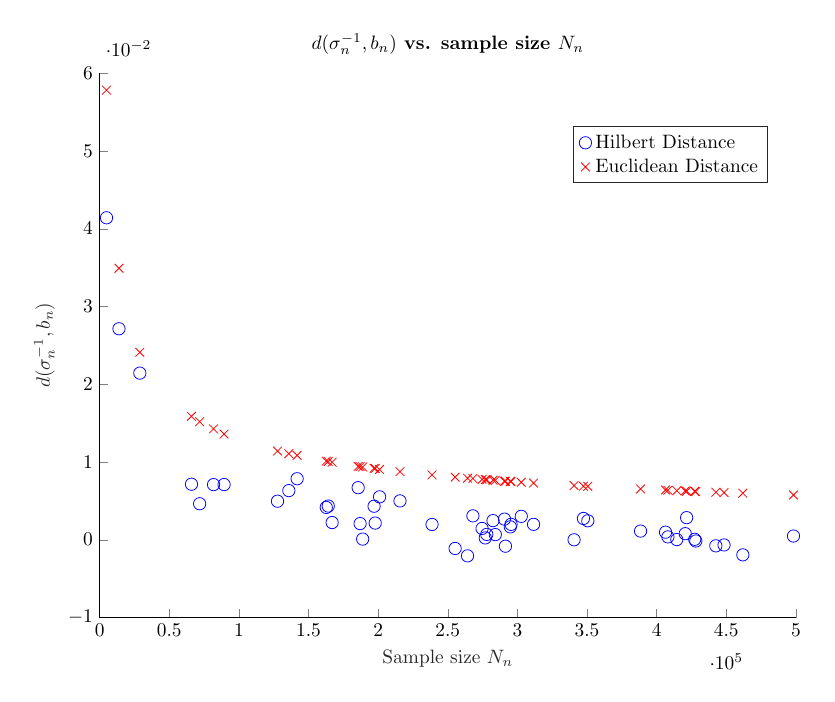
\begin{tikzpicture}[scale = .7]

\begin{axis}[%
width=4.973in,
height=3.888in,
at={(0.834in,0.525in)},
scale only axis,
xmin=0,
xmax=500000,
xlabel style={font=\color{white!15!black}},
xlabel={Sample size $N_n$},
ymin=-0.01,
ymax=0.06,
ylabel style={font=\color{white!15!black}},
ylabel={$d(\sigma^{-1}_n,b_n)$},
axis background/.style={fill=white},
title style={font=\bfseries},
title={$d(\sigma_n^{-1} , b_n)$ vs. sample size $N_n$},
axis x line*=bottom,
axis y line*=left,
legend style={at={(.68,.85)}, anchor=west, legend cell align=left, align=left, draw=white!15!black},
]

\addplot[only marks, mark=o, mark options={}, mark size=3.180pt, draw=blue] table[row sep=crcr]{%
x	y\\
185654	0.00669821643582239\\
461919	-0.00194082366533434\\
13881	0.0271349448909549\\
347441	0.00273861163016988\\
294926	0.00165898367749918\\
284160	0.000665515638284928\\
65940	0.00714178042487273\\
164165	0.00433545683243485\\
302796	0.00301026969263965\\
406401	0.000973568780387476\\
188891	8.56925149069643e-05\\
215693	0.00499739716604691\\
141821	0.00784764005809632\\
448418	-0.000668346663740666\\
350587	0.00243824401822285\\
268060	0.00307267881580029\\
278032	0.000686757672117151\\
255289	-0.00112088430282066\\
276953	0.000237919846155388\\
135868	0.0063204121774592\\
187057	0.00207727993409978\\
264210	-0.00206993361413214\\
290745	0.00265365765192809\\
340718	-5.9537670431143e-06\\
408106	0.000369722136538977\\
442518	-0.000781879719060814\\
166964	0.00221571913204337\\
421545	0.00284320005159473\\
311615	0.00198158270015289\\
197887	0.00214526160425017\\
428145	-0.000162215650257437\\
238711	0.00196677377317525\\
414489	2.44849030291002e-05\\
291437	-0.000829678691013056\\
197088	0.00431304005432322\\
89377	0.00709862858045795\\
388458	0.00111572158314997\\
295440	0.00197997267388959\\
420523	0.000780474323874054\\
498286	0.000479633145504096\\
4930	0.0414055765697148\\
201038	0.00551830560930839\\
274642	0.00145336990897321\\
81797	0.00709088105925166\\
162750	0.00416016433921489\\
282509	0.00246178693446355\\
127740	0.00495888442610629\\
427344	5.60809200664666e-05\\
28852	0.0214301089453041\\
71802	0.00463015133986612\\
};
\addlegendentry{Hilbert Distance};

\addplot[only marks, mark=x, mark options={}, mark size=3.180pt, draw=red] table[row sep=crcr]{%
x	y\\
185654	0.0094325253120403\\
461919	0.00599305595208928\\
13881	0.0349149558250945\\
347441	0.006892850280004\\
294926	0.00749921720669556\\
284160	0.00763770291802395\\
65940	0.0158790580679202\\
164165	0.0100573696892928\\
302796	0.0073975686357452\\
406401	0.00639930136381924\\
188891	0.00935982342673795\\
215693	0.00876493822499141\\
141821	0.0108563841719144\\
448418	0.00607358019476551\\
350587	0.00686605979052986\\
268060	0.00788141750048222\\
278032	0.00771931031484074\\
255289	0.00805283015528211\\
276953	0.00774517412816496\\
135868	0.0110653597390213\\
187057	0.00942161940914911\\
264210	0.0079186462583656\\
290745	0.00752260942754111\\
340718	0.00697044450195269\\
408106	0.00636490880463546\\
442518	0.00610618431953571\\
166964	0.00996997427611699\\
421545	0.00624909251477234\\
311615	0.0072897210875988\\
197887	0.00917547900585788\\
428145	0.00618961802899384\\
238711	0.00834048653268987\\
414489	0.00631346151232045\\
291437	0.00752596027630547\\
197088	0.00918728723416085\\
89377	0.0135880555333526\\
388458	0.00652981307302403\\
295440	0.0074917537895146\\
420523	0.00627302958876728\\
498286	0.005759280075179\\
4930	0.0578194744732125\\
201038	0.00904298400436458\\
274642	0.00775525119793726\\
81797	0.0142618731367437\\
162750	0.0101130467723554\\
282509	0.00765971524118242\\
127740	0.0114068725648567\\
427344	0.00622912051602129\\
28852	0.0241031539282733\\
71802	0.0151705630937243\\
};
\addlegendentry{Euclidean Distance};

\end{axis};

\end{tikzpicture}%
	
	\caption[Plot of distances \( d(\gs_F^{-1},|b_F|) \) for various \( F \) ]{Linear regression was performed on the curves in figure \ref{fig:convLines} to get equations of the form \( \log(a_n) = b_{F}n +c_{F} \) for various \( F \).  Then the max singular value \( \gs_F \) for the same \( F \) was computed.  The scatter plot above shows the distances \( d(\gs_F^{-1},|b_F|) \) plotted against \( N \), the number of columns of \( F \) for two different distances.
	
%	The $x$-axis reprents the sample size \( N_n \) of the $n$-th run, and the $y$-axis the difference between the slopes from figure \ref{fig:convLines}a. The red and blue 
	 }\label{fig:residuesVsamplesize}
\end{figure}

\begin{figure}[h]
	\subcaptionbox{Plot of \( a_n \) for several \( F \)}{
		\includegraphics[scale=1]{chapter5/log_dist_nVn}
	}
	\subcaptionbox{Plot of \( \ge_n \) for several \( F \)}{
		\includegraphics[scale=1]{chapter5/log_err_nVn}
	}
	
	\caption[Plots of distances and convergence errors for various \( F \) ]{The two plots show \( a_n \) and \( \ge_n \) for euclidean distance. Each individual curve represents a different parameter matrix \( F \).}\label{fig:convLines}
\end{figure}

Given the lines formed by \( a_n \) for a particular matrix \( F \), let \( b_F \) be the slope of that line. For the same \( F \) let \( \gs_F \) be the largest singular value of \( F \). Figure \ref{fig:residuesVsamplesize} shows a scatter plot of \( \gs_F^{-1}+b_F \) compared to \( N \), the number of columns of \( F \), for two different runs of experiment \ref{exper:conv}.  Notice that as \( N \) increases the residues go to zero like \( \frac{1}{\sqrt N} \). This shows an expected relationship between convergence rate and sample size, or batch size in the case of neural network training.

While it is clear that the curves in figure \ref{fig:convLines} are eventually linear, in the first few steps many of the curves shrink much faster than linear. This suggests that most of the convergence happens in the first few iterations. It also encourages setting the hyperparameter \( C \) for the \RS layer to a small value. As will be seen in section \ref{sect:GMMresults}, optimal values for \( C \) are less than 10.

%Future work may seek to better understand eigenvalues of \( \nabla^2\ell_{F} \) to set a reasonable bound on convergence behavior.\Ryan{PTS}
%
%\Ryan{Keep this discussion here to provide motivation for setting \( C<10 \) or so. Explain a bit why \( C=1,2 \) are so effective}

%\Ryan{Can I add experimental computation of Lyapunov exponents? They should all be the same sign. time worries?yes. save for future work!}

%\Ryan{If \( R_F \) is Lipschitz, then rate is linear? What is quadratic convergence?  Results of experiment \ref{exper:conv} suggest better than linear (at least initially). as per comment by marek below, iteration should be quasi newton (not linear, but not quadratic.)  }

%\Marek{%
%  Quadratic convergence is a quadratic rule for error. If
%  $\epsilon_n = \|R_F^n(\pi)-\hat{\pi} \|$ then
%  $\epsilon_{n+1} \sim c\cdot\epsilon_n^2$. But this would require
%  $DR_F(\hat\pi)=0$ which clearly is not the case. Quadratic
%  convergence is attainable by applying Newton's method to the
%  equation $R_F(\pi)=\pi$. Kantorovich is about this kind of
%  accelleration of the speed of convergence. Methods yielding
%  $\epsilon_{n+1} \approx c\cdot\epsilon_n^\alpha$, $1<\alpha<2$ are
%  called quasi-Newton. If you use $(I-D_FR)^{-1}$ then the method is
%  Newton and yields quadratic convergence. If you are approximating
%  $(I-D_FR)^{-1}$, you shuld get
%  quasi-Newton.\\
%  (BELOW IS STANDARD STUFF FROM BOOKS LIKE NITECKI OR ABRAHAM-ROBBIN.)\\
%  So, how to you apply Newton to the equation $R(\pi)=\pi$?  You
%  linearize $R$ at the point $\pi$:
%  \begin{align*}
%    \hat\pi =& R(\hat\pi) = R(\pi) + DR(\pi)(\hat\pi-\pi)\\
%             &= R(\pi) + DR(\pi)(\hat\pi-\pi),\\
%  \end{align*}
%  Subtract $\pi$ from both sides and get
%  \begin{align*}
%    \hat\pi-\pi &= (R(\pi)-\pi) + DR(\pi)(\hat\pi-\pi),\\
%    (I-DR(\pi))(\hat\pi-\pi) &= (R(\pi)-\pi),\\
%    \hat\pi - \pi &= (I-DR(\pi))^{-1}(R(\pi)-\pi),\\
%    \hat\pi &= \pi + (I-DR(\pi))^{-1}(R(\pi)-\pi).\\
%  \end{align*}
%  Now define
%  \[ S(\pi) = \pi + (I-DR(\pi))^{-1}(R(\pi)-\pi) \]
%  Iterating $\pi_{n+1}=S(\pi_n)$ yields quadratic convergence. In particular,
%  $DS(\hat\pi) = 0$.}
%
%
%\Marek{Convergence cannot be better then linear for plain fixed point
%  iteration $\pi_{n+1}=R(\pi_n)$, unless $DR(\hat\pi)=0$. To have
%  convergence at all, it is necessary that $spectrum(DR(\hat\pi)$ is
%  contained in the unit circle, and for linear convergence it is
%  required to be strictly in the unit circle, i.e. the spectral radius
%  needs to be $<1$. Linear convergence is defined as
%  $\epsilon_{n+1}\sim \lambda \epsilon_n$, where $\lambda<1$.}
\FloatBarrier